\documentclass[12pt, a4paper]{article}

\usepackage[spanish]{babel}

\usepackage{amsmath} % Escritura mejorada de fórmulas matemáticas
\usepackage{graphicx} % Inserción de gráficos
\usepackage{algorithm}
\usepackage{algpseudocode}

\usepackage[colorlinks=true, citecolor=blue]{hyperref}



\title{Crucigrama CBD}
\author{Pedro González Marcos}
\date{27 de Mayo 2024}

\begin{document}

\maketitle

\tableofcontents

\section{Introducción}

La idea de este trabajo surge principalmente de una necesidad doble
que tenía antes de los exámenes de la primera convocatoria de CBD.

Hacer el proyecto de CBD y prepararme para el tipo test de la asignatura.

Entonces se me ocurrió implementar una aplicación de crucigrama que
tematizada en la asignatura. 


\section{Crucigrama}

Para poner en contexto al que no esté familiarizado con este juego.
El crucigrama es un pasatiempo donde tienes que introducir palabras
en una cuadrícula siguiendo las pistas proporcionadas por el crucigramista.

Lo que hace a un crucigrama divertido, es el reto intelectual que plantea
a la persona.

Aunque un crucigrama pueda parecer injusto a priori, si no te sabes
una solución puedes intentar sacar la palabra resolviendo otras pistas.
Esto hace que puedas seguir avanzando en el pasatiempo. Conforme vas
rellenado el crucigrama llega un punto que puedes intuir la palabra.

Podemos ejemplo, en Estados Unidos publican diariamente en el periódico
1 crucigrama. Los del lunes son los más sencillos y más pequeños (11x11) y
los domingos son más complicados siendo más grandes (21x21)  y con pistas
más crípticas.


\subsection{Cuadrícula}

Podemos distinguir en la cuadrícula del crucigrama 2 elementos:

\begin{itemize}
	\item Las celdas negras
	\item Las celdas blancas
\end{itemize}

En las celdas negras no se puede escribir nada y sirven para delimitar
la longitud de las palabras. Los crucigramistas, suelen jugar con los bloques
para crear sus crucigramas. Pueden ponerlas por conveniencia al  o por simple
estética. En general dependiendo donde la coloquen, el crucigrama tendrá más
o menos palabras.

En las celdas blancas, por el contrario, es donde tenemos que poner las
respuestas a las pistas. 

Además, si nos fijamos en el crucigrama de la figura
\ref{fig:americanXword}, podemos ver que algunas celdas tienen numeración. Esto tiene
que ver con la forma de dar pistas en el crucigrama. Exista la variante numerada
de la figura \ref{fig:americanXword} y la variante de la figura \ref{fig:xwordESP}

\begin{figure}[p]
	\centering
	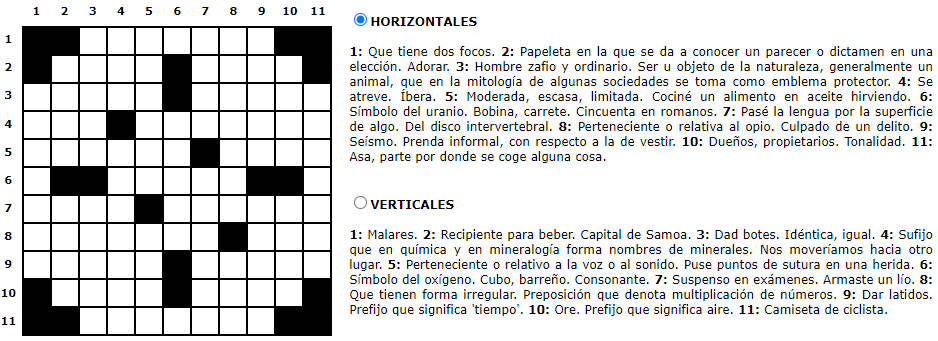
\includegraphics[width=\textwidth]{img/xword-weird.png}
	\caption{Crucigrama numerando filas y columnas}
	\label{fig:xwordESP}
\end{figure}

\begin{figure}[p]
	\centering
	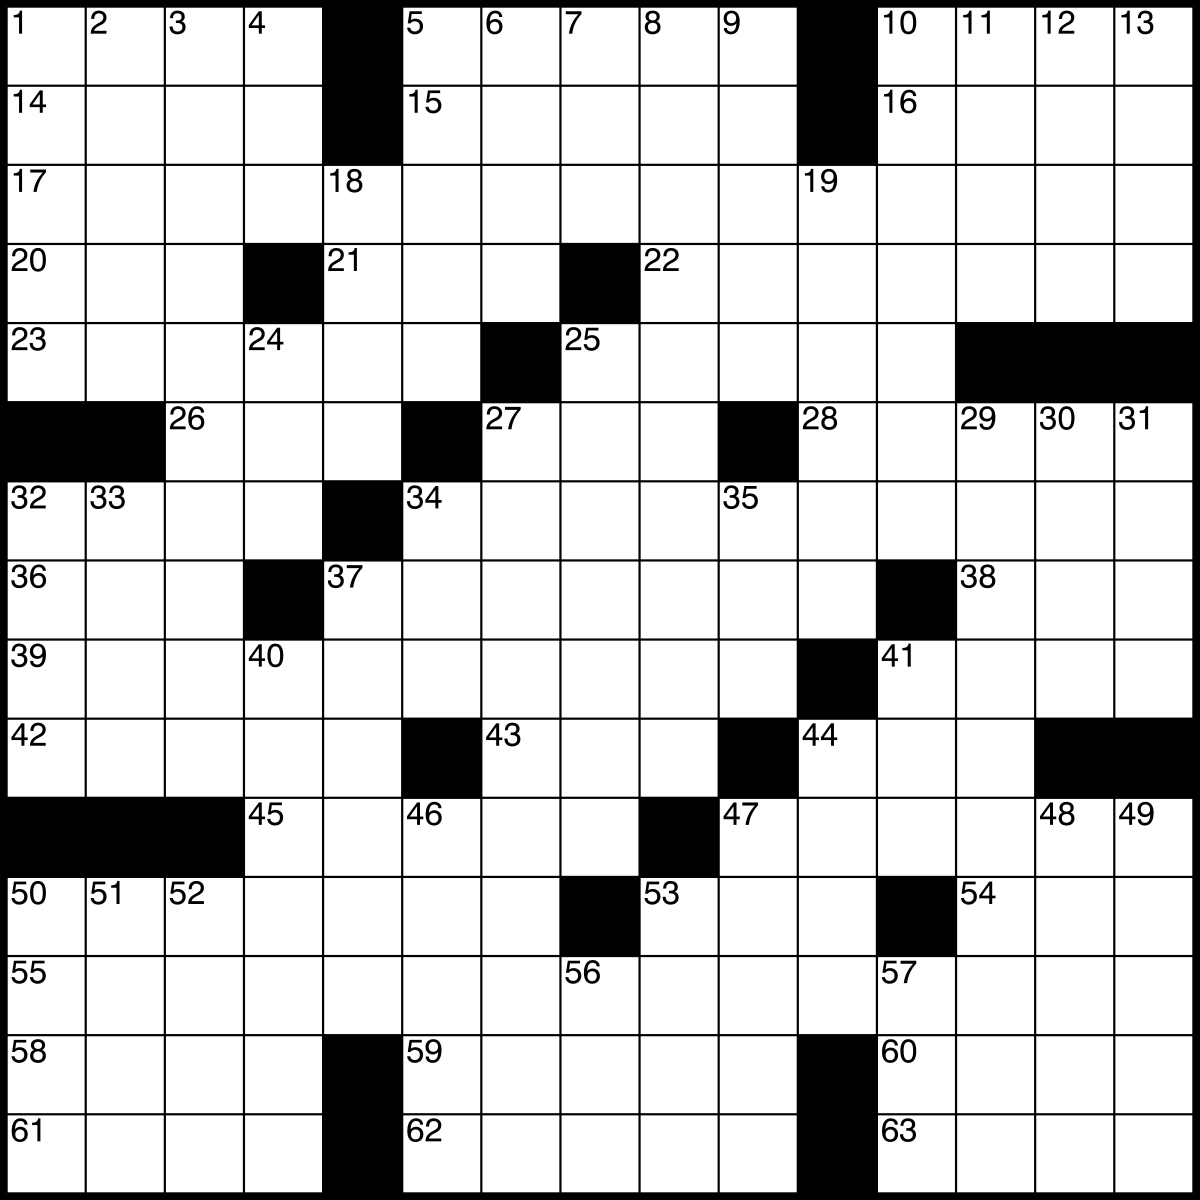
\includegraphics[width=0.7\textwidth]{img/CrosswordUSA.png}
	\label{fig:americanXword}
	\caption{Crucigrama vacío numerado}
\end{figure}


\subsection{Pistas}

Un crucigrama está formado por palabras en vertical y en horizontal. Para
solucionar el crucigrama se da una serie de pistas. Estas pistas pueden
referenciarse en el crucigrama de 2 formas distintas.

\begin{itemize}
	\item Coodernadas: Se numeran las filas y las columnas del crucigrama. Por cada palabra
	que haya en una fila o columna se añade a la lista de pistas horizontales o
	verticales en la fila o columna que toca. Por ejemplo en la figura \ref{fig:xwordESP}
	la fila 3 tiene dos palabras en una misma fila, por lo que en las pistas
	horizontales podemos ver separado por puntos las dos pistas.
	\item Numeración de casillas: Se ponen número a las celdas que empiecen una palabra ya
	sea en horizontal, en vertical o ambas. Puede ver como funciona el algortimo
	para detectar etiquetas en la sección \ref{sec:algo}.
\end{itemize}


\section{Modelo de datos}

Para modelar este pasatiempo necesitamos modelar al menos 3 objectos:

\begin{itemize}
	\item La cuadrícula
	\item La solución
	\item Las pistas
\end{itemize}

\subsection{Cuadrícula}

Viendo la figura \ref{fig:americanXword} las celdas están dispuestas en filas
y columnas.

En MongoDB podemos guardar listas de cualquier objeto que se nos ocurra, por
lo que vamos a representar la cuadrícula con una lista de filas y cada fila
con una lista de celdas. 

Para representar las celdas y los bloques podemos simplemente modelarlo
como un atributo Booleano que tenga dos estados. Este atributo que llamaremos
\verb*|dark|, es verdadero si la celda es un bloque y falso si es una celda
en blanco.

Adicionalmente, dejaremos un atributo llamado \verb*|solution| que contendrá una
cadena de un caracter, es decir, una letra que será la solución de la celda.

Una vez modelado todos los componentes de la cuadrícula tenemos que elegir de
qué forma vamos a presentar las pistas a los usuarios. En este caso se ha optado
por la estrategia de numerar las casillas.

Si implementamos esta estrategia las celdas tendría un atributo opcional para
guardar el número de la casilla. Es importante destacar que no todas las casillas
tendrán número sólo aquellas que comiencen una palabra. Por ejemplo si nos fijamos
en la casilla 3,2 de la figura \ref{fig:xwordNYT} vemos que no tiene ningún número
asignado ya que la casilla 3,2 ya pertenece a la palabra 6H y 1D.

Además para que los usuarios puedan ver fácilmente que palabra están solucionando,
otros portales de pasatiempos como el New York Times suelen colorear de otro color
la cuadrilla como podemos ver en la figura \ref{fig:xwordNYT}.

Podemos modelar esto con dos atributos opcionales \verb*|across| y \verb*|down|
que tendrán una etiqueta de la palabra horizontal y vertical a la que pertenecen.
Estos dos atributos opcionales no pueden ser simultáneamente nulos ya que la celda
tendrá que pertenecer al menos a una palabra del crucigrama ya sea en horizontal
o en vertical. Si, embargo, se puede dar la situación de que una celda no pueda
pertenezca a una palabra en horizontal o viceversa. El algoritmo encargado de 
etiquetar las celdas es el descrito en la sección \ref{sec:algo}.


Al final el aspecto de la cuadrícula modelada como un documento 
sería el siguiente tomando como ejemplo el de la figura \ref{fig:xwordNYT}.

\begin{verbatim}
[
  [
   { 
   	dark: true
   	solution: "."
   },
   {
   	dark: false,
   	solution: "V",
   	label: "1",
   	across: "1A",
   	down: "1D" 
   },
   {
   	dark: false,
   	solution: "I",
   	label: "2",
   	across: "1A",
   	down: "2D"
   },
   {
   	dark: false,
   	solution: "P",
   	label: "3",
   	across: "1A",
   	down: "3D"
   },
  ],
  ...,
]
\end{verbatim}

\subsection{Pistas}

Otra parte fundamental a modelar del crucigrama son las pistas. Como vemos
en la figura \ref{fig:xwordNYT} situada a la derecha de la cuadrícula podemos
ver dos columnas con pistas en horizontal y en vertical.

Siguiendo este mismo diseño, podemos pensar en una pista como un objeto \verb*|Clue|
con dos atributos su etiqueta \verb*|label| y su texto asociado \verb*|hint|
como podemos ver en el diagrama \ref{fig:datamodel}.

Para formar el documento final que contiene las pistas del crucigrama simplemente
tenemos dos atributos con una lista de pistas horizontales y verticales.

El documento final que modela a las pistas se vería de la siguiente forma.

\begin{verbatim}
	{
	  "across": [
	    {
	      "label": "1A",
	      "hint": "Someone who might have a special line to the entrance"
	    },
	    ...
	  ]
	  "down": [
	    {
	      "label":"1D",
	      "hint": "Physicist for whom an electrical measurement is named"
	    },
	    ...
	  ]
	}
\end{verbatim}


a un documento podemos pensar que es un objeto con dos propiedades las pistas
en horizontal y en vertical. Estos campos van a tener una lista de pistas que
tiene dos atributos la etiqueta de la pista en el diagrama \verb*|label|
por ejemplo \verb*|1A| y el campo \verb*|hint| que es el texto asociado.

\begin{figure}[p]
	\centering
	\label{fig:datamodel}
	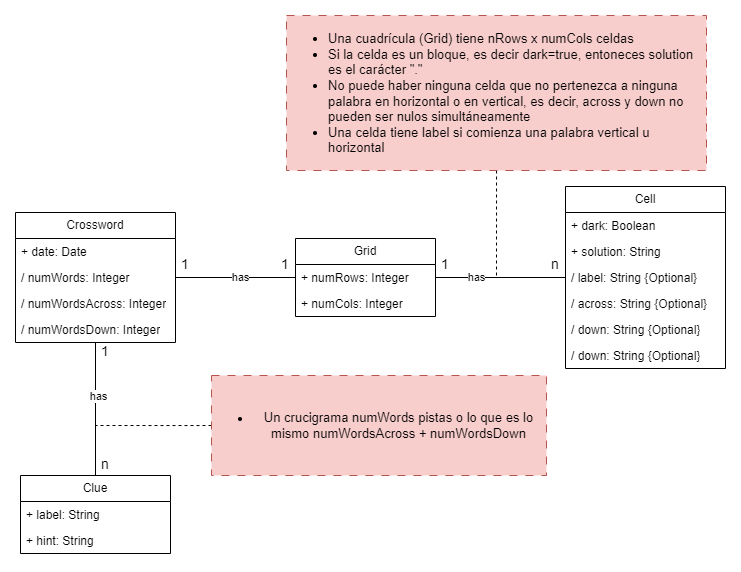
\includegraphics[width=0.8\linewidth]{img/datamodel.png}
	\caption{Modelo conceptual del crucigrama}
\end{figure}


\begin{figure}[p]
	\centering
	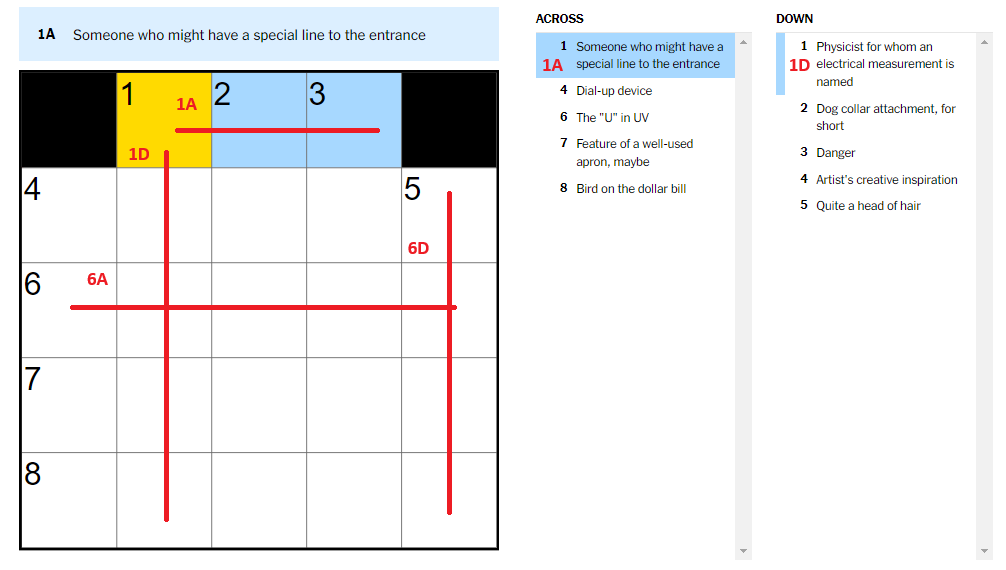
\includegraphics[width=0.8\textwidth]{img/new-york-times-xword.png}
	\caption{Crucigrama con celdas numeradas}
	\label{fig:xwordNYT}
\end{figure}

\subsection{Crucigrama}

Con la cuadrícula y las pistas ya tenemos un crucigrama funcional que podemos
representar en un documento al que le vamos a añadir un atributo fecha
\verb*|date| que utilizaremos como clave alternativa para modelar la publicación
de un crucigrama diario. 

Además también podemos añadir al modelo del crucigrama 3 atributos derivados, el número de
palabras horizontales, el número de palabras verticales y el número total de 
palabras \ref{fig:datamodel}.

El documento final tendría la siguiente pinta si juntamos el JSON que modela
la cuadrícula y las pistas. Para no repetir el mismo JSON anterior se ha puesto
una elipsis.

\begin{verbatim}
	{
		"date": { "$date": "2024-06-24T00:00:00.000Z" },
		"numRows": 5,
		"numCols": 5,
		"numWords": 10,
		"numWordsAcross": 5,
		"numWordsDown": 5,
		"crossword": [...]
		"clues": {
			across: [...]
			down: [...]
		}
	}
\end{verbatim}

\subsection{Algoritmo} \label{sec:algo}

En esta sección describiremos brevemente el algoritmo utilizado para detectar
las etiquetas que tiene el crucigrama. Está pensado para trabajar
con crucigramas Americanos \cite{XwordRules} que tienen una serie de reglas
como:

\begin{itemize}
	\item Las palabras están formadas por al menos 3 letras.
	\item El crucigrama debe ser simétrico si lo rotamos 180º, es decir si lo 
	rotamos debe coincidir las celdas originales
\end{itemize}

El algoritmo detectará una palabra, si al menos su longitud es de tres caracteres.

A continuación se muestra el pseudocódigo \cite{pseudocode} que describe al
algoritmo:

\begin{figure}[h]
	\centering
	\label{fig:detectLabels}
	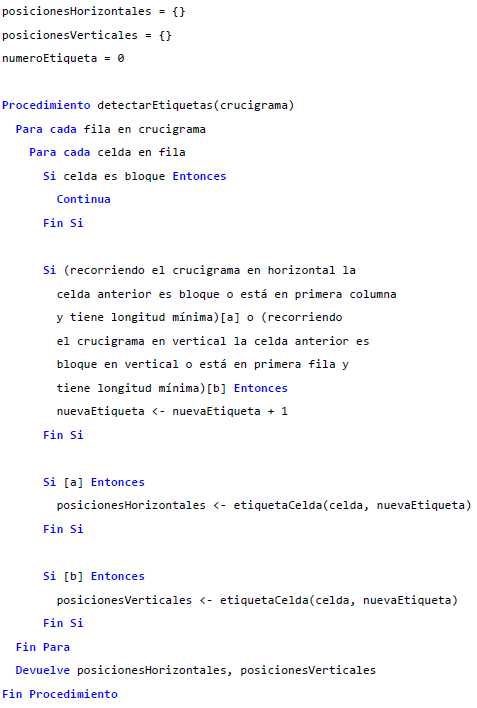
\includegraphics[width=0.7\linewidth]{img/pseudocode.png}
	\caption{Algoritmo detector de etiquetas}
\end{figure}


\section{Marco de trabajo}

Con el modelo de datos terminado ya podemos pasar un crucigrama a un
documento en EJSON \cite{EJSON} (archivo JSON en el que se especifican
los tipos de datos de MongoDB). No obstante, el modelo planteado es bastante largo
como para que una persona se ponga a escribir un JSON a mano.

Por esta razón se ha desarrollado el marco del proyecto un script  que transforma
una cuadrícula en un formato personalizado en un documento EJSON (Paso 1 figura
\ref{fig:framework}). Luego importaremos el documento resultante a la BBDD (Paso 2
\ref{fig:framework}).

  
\begin{figure}[h!]
	\centering
	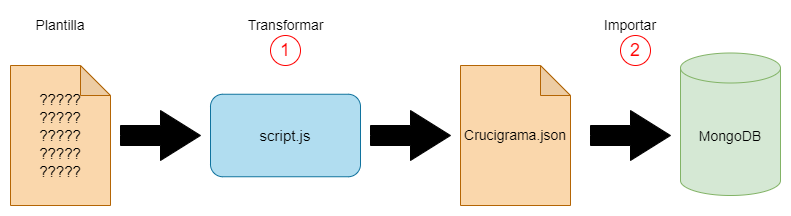
\includegraphics[width=\linewidth]{img/framework}
	\caption{Transformación del formato de texto a JSON que puede leer MongoDB}
	\label{fig:framework}
\end{figure}

El formato personalizado elegido para representar este pasatiempo es el de
la página Words Up? \cite{wordsUp} que tiene un gran librería de crucigramas
hechos

El formato propuesto por la página es el siguiente:

\begin{itemize}
	\item Las bloques se representan con un punto.
	\item Las celdas en blanco se representan con un interrogante.
	\item El número de filas del crucigrama es el número de líneas.
	\item El número de columnas del crucigrama es la longitud de caracteres de una
	línea. La longitud debe ser consistente en todas las líneas del crucigrama. Es
	decir todas las líneas deben tener la misma longitud de caracteres.
	\item El saldo de línea \verb*|\n| o \verb*|\r\n| indica la terminación
	de una fila y el comienzo de la siguiente.
	\item Cualquier carácter que no sea un punto, un interrogante o un salto de línea
	es inválido.
	\item No se admiten líneas en blanco
\end{itemize}

Por ejemplo en la figura \ref{fig:xwordCustomFormat} podemos ver el formato de archivo
propuesto. 

\begin{figure}[t]
	\centering
	\label{fig:xwordCustomFormat}
	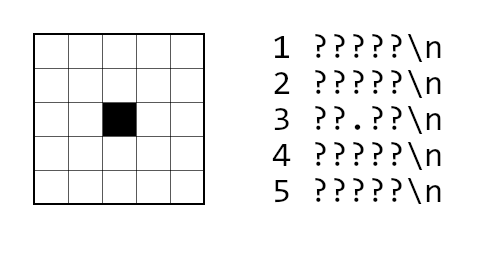
\includegraphics[width=0.7\linewidth]{img/formato.png}
	\caption{A la izquierda un crucigrama con 5 filas y 5 columnas.
		A la derecha la representación del crucigrama en un archivo de texto}
\end{figure}

Este formato facilita de crear las plantillas Siendo la alternativa de JSON
menos legible y mucho más verboso.

Una vez ya tenemos la cuadrícula, la solución pensada y las pistas escritas
le damos la cuadrícula al script y el programa se encarga de crearnos la plantilla
en EJSON \cite{EJSON}.

Ya con el archivo en JSON creado, tiene que escribir la solución del crucigrama en
la cuadrícula, que es simplemente rellenar donde ponga \verb*|<SOLUTION>| el caracter 
de la palabra correspondiente. Después en la sección \verb*|clues| tiene que rellenar 
las pistas horizontales y verticales. 

Es importante mencionar que la fecha que saca el script está en EJSON \cite{EJSON}
un formato que permite importar datos de diferentes tipos a MongoDB. En este caso
si quere importar una fecha a MongoDB. Tiene que escribir lo siguiente: 

\begin{verbatim}
	"date": { "$date": "2024-06-22T00:00:00.000Z" }
\end{verbatim}

Para ejecutar el script por favor consulte el README del repositorio \cite{repositorio}
o el Anexo \ref{sec:Anexo} de este documento.

Una vez que tenemos el JSON definitivo podemos importar el JSON en la instancia de
MongoDB utilizando el comando mongo


\subsection{Express}

En vez de utilizar los métodos nativos del servidor de http que expone node se ha
utilizado la librería de npm \verb*|express| que nos ofrece una abstracción para 
implementar rutas de una API.

Se ha organizado los siguientes endpoints:

\begin{verbatim}
	1 GET  /crosswords
	2 GET  /crosswords/AAAA-MM-DD
	3 POST /crosswords/AAAA-MM-DD/solution
\end{verbatim}

Para listas todos los crucigramas que hay en la BBDD hay que hacer una llamada http
de tipo GET al primer \textit{endpoint} expuesto por la API.

Para consultar una crucigrama por su fecha de publicación simplemente tiene que hacer
una llamada tipo GET al segundo \textit{endpoint} poniendo en la url por parámetro
el año, el mes y el dia. Por ejemplo:

\begin{verbatim}
	GET /crosswords/2024-06-24
\end{verbatim}

Para comprobar si el crucigrama que ha hecho el usuario es correcto, se envía la 
solución del usuario en el cuerpo de la petición al servidor.

El formato de la solución que acepta este \textit{endpoint} lo podemos ver en
el siguiente ejemplo.

Si tenemos el crucigrama solucionado:

\begin{verbatim}
	CBD
	B..
	D..
\end{verbatim}

La solución al crucigrama es la cadena de caracteres \verb|CBDB..D..|.

Si una persona tiene lo siguiente como solución al crucigrama

\begin{verbatim}
	CBD
	C..
	O..
\end{verbatim}

Enviará al servidor la solución \verb*|CBDC..O..|. Si no coinciden las soluciones,
el servidor responde con un código de estado 400.

\subsection{MongoDB}

Para poder comparar las soluciones del usuario y del crucigrama se ha utilizado
una agregación de MongoDB para sacar la cadena solución del crucigrama \ref{fig:reducequery}.

La idea básica con un \verb*|reduce| concatenar los caracteres solución de una fila
y luego concatenar las cadenas de todas las filas, obteniendo así la cadena solución.

\begin{figure}[h!]
	\centering
	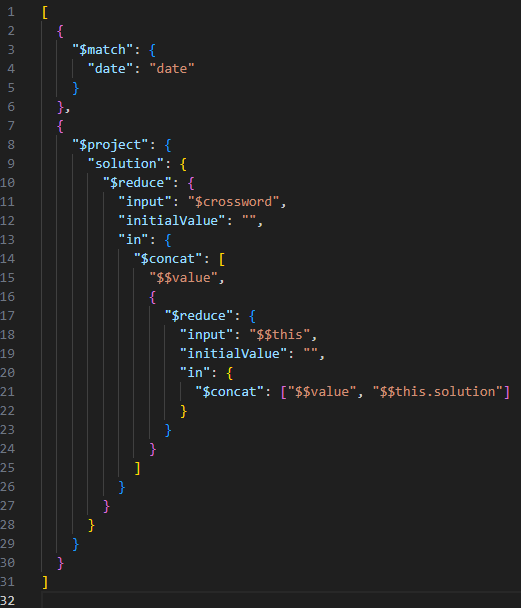
\includegraphics[width=\linewidth]{img/reduceQuery}
	\caption{Agregación para obtener solución del crucigrama.}
	\label{fig:reducequery}
\end{figure}

\section{Conclusiones}

\section{Anexo} \label{sec:Anexo}

\subsection{Prerequisitos}

\begin{itemize}
	\item NodeJS 20.X.X o superior (https://nodejs.org/en/)
	\item Docker Desktop (Windows, https://www.docker.com/products/docker-desktop/),
	Docker Engine (Linux, https://docs.docker.com/engine/install/)
\end{itemize}

Para arrancar tanto el frontend como el backend se necesita alguna distribución
de NodeJS instalada. Para arrancar el backend hay que seguir los siguientes pasos:

\begin{verbatim}
Antes de arrancar el back necesita que el driver de mongodb para
express se conecte a una instancia en el ordenador,
si utiliza docker:
> docker run --name xword -p 27017:27017 -d mongo:latest

Una vez arrancada la BBDD puede arrancar el backend
	
Sitúese en la capeta back
> cd back
> npm install
> npm build  # Crea una carpeta dist en el que se encontrarán
los archivos .js requeridos para ejecutar el servidor de express

Después de arrancar mongo ya está en condiciones para arrancar
el servidor de express
> node dist/index.js
\end{verbatim}

Para arrancar el frontend tiene que situarse en la carpeta front y ejecutar

\begin{verbatim}
> cd front
> npm install
> npm run dev
\end{verbatim}

\subsection{Script}

El script tiene los siguientes parámetros posicionales:

\begin{itemize}
	\item Número de filas
	\item Número de columnas
	\item Ruta del archivo donde se encuentra la cuadrícula con el formato
	\ref{fig:xwordCustomFormat} esperado.
\end{itemize}

Para ejecutar el script primero tendrá que hacer los siguientes pasos:

\begin{verbatim}
	> cd back
	> npm install (Opcional si ya ha instalado los node_modules)
	> npm build (Se crea un carpeta dist con script.js)
\end{verbatim}

Ejemplo de uso:

\begin{verbatim}
	Windows:
	> node dist\script.js 11 11 --grid=.\crossword\example.txt
	Linux:
	> node ./dist/script.js 11 11 --grid=./crossword/example.txt
\end{verbatim}

\begin{thebibliography}{100}
	\bibitem{XwordRules} Shortz, W. (s.f). \textit{Real Rules of the Puzzle}.
	BarelyBad. https://barelybad.com/xwdrulesreal.htm
	\bibitem{pseudocode} Wikipedia (s.f). \textit{Pseudocódigo}. Wikipedia. https://es.wikipedia.org/wiki/Pseudoc\%C3\%B3digo
	\bibitem{OneLook} OneLook (s.f). \textit{OneLook}. https://onelook.com/
	\bibitem{wordsUp} Words Up Games (s.f). \textit{Grid Library for Crossword 
	Compiler and Sympathy}. Words Up Games. https://wordsup.co.uk/grid-libraries.php
	\bibitem{EJSON} MongoDB (s.f). \textit{EJSON}. MongoDB. https://www.mongodb.com/docs/mongodb-shell/reference/ejson/
	\bibitem{repositorio} González, P. (26 de Mayo de 2024). \textit{crossword}. crossword.
	https://github.com/pgmarc/crossword
	\bibitem{repoDic} Duenas, J (). \textit{diccionario-espanol-txt}. Diccionario español.
	https://github.com/JorgeDuenasLerin/diccionario-espanol-txt
\end{thebibliography}



\end{document}